\documentclass[format=sigconf]{acmart}
\usepackage[utf8]{inputenc}
\usepackage{enumitem}
\usepackage{float}
\usepackage[labelfont=bf,textfont=md]{caption}
\usepackage{graphicx}
\usepackage{xcolor}
\usepackage{minted}
\usepackage{hyperref}
\usepackage[all]{hypcap}
\usemintedstyle[glsl]{default}
\usemintedstyle[common-lisp]{default}
\newmintinline[code]{text}{}
\bibliographystyle{plainnat}

\hypersetup{
  colorlinks,
  linkcolor={red!50!black},
  citecolor={blue!50!black},
  urlcolor={blue!80!black}
}

\newlist{step}{enumerate}{10}
\setlist[step]{label*=\arabic*.,leftmargin=2em}

\acmConference[ELS'19]{the 12th European Lisp Symposium}{April 01--02 2019}{%
  Genova, Italy}
\acmISBN{978-2-9557474-3-8}
\acmDOI{10.5281/zenodo.2636508}
\setcopyright{rightsretained}
\copyrightyear{2019}

\begin{document}

\title{Shader Pipeline and Effect Encapsulation using CLOS}

\author{Nicolas Hafner}
\affiliation{%
  \institution{Shirakumo.org}
  \city{Zürich}
  \country{Switzerland}
}
\email{shinmera@tymoon.eu}

\begin{abstract}
  Modern real-time graphics make use of a lot of tricks in order to produce stunning visuals. Many of these tricks require separate rendering passes, as well as separate rendering logic for each pass. These passes are then combined in a variety of ways in order to produce a final image. The interaction between such a rendering pass and the objects it draws, as well as the interaction between multiple passes within a pipeline can become quite complex. Often times, in order to handle this complexity, the passes and objects are generalised, and the render logic is controlled almost entirely by either the object or the pass. We present a new method of representing objects, passes, and pipelines, which allows a modular encapsulation of effects and rendering behaviour, as well as object-oriented composition through inheritance. We make use of CLOS' multiple inheritance, multimethods, and standard method combination to form extensible protocols that allow this new method. We also make use of the MOP, in order to introduce additional metadata to classes.
\end{abstract}

\begin{CCSXML}
  <ccs2012>
  <concept>
  <concept_id>10011007.10010940.10010971.10010972.10010979</concept_id>
  <concept_desc>Software and its engineering~Object oriented architectures</concept_desc>
  <concept_significance>500</concept_significance>
  </concept>
  <concept>
  <concept_id>10011007.10010940.10010971.10011682</concept_id>
  <concept_desc>Software and its engineering~Abstraction, modeling and modularity</concept_desc>
  <concept_significance>500</concept_significance>
  </concept>
  <concept>
  <concept_id>10011007.10011006.10011066.10011067</concept_id>
  <concept_desc>Software and its engineering~Object oriented frameworks</concept_desc>
  <concept_significance>300</concept_significance>
  </concept>
  <concept>
  <concept_id>10010147.10010371</concept_id>
  <concept_desc>Computing methodologies~Computer graphics</concept_desc>
  <concept_significance>300</concept_significance>
  </concept>
  <concept>
  <concept_id>10011007.10011006.10011041.10011688</concept_id>
  <concept_desc>Software and its engineering~Parsers</concept_desc>
  <concept_significance>100</concept_significance>
  </concept>
  </ccs2012>
\end{CCSXML}

\ccsdesc[500]{Software and its engineering~Object oriented architectures}
\ccsdesc[300]{Software and its engineering~Abstraction, modeling and modularity}
\ccsdesc[300]{Software and its engineering~Object oriented frameworks}
\ccsdesc[300]{Computing methodologies~Computer graphics}
\ccsdesc[100]{Software and its engineering~Compilers}

\keywords{Common Lisp, OpenGL, GPU, CLOS, Object Orientation}

\maketitle

\newpage

\def\abovecaptionskip{1pt}
\def\listingautorefname{Listing}
\def\figureautorefname{Figure}

\section{Introduction}\label{introduction}
Modern graphics systems such as OpenGL Core and DirectX offer a lot of customisation to the programmer. Particularly, in order to render an image, they allow the programmer to supply code fragments (shaders) that are run directly on the GPU. These code fragments fill in steps of a fixed rendering pipeline that is executed on the GPU in order to transform vertex data into the pixels of an image. The pipeline for OpenGL is illustrated in \autoref{fig:opengl-pipeline}. \\

\begin{figure}[h]
  \begin{center}
    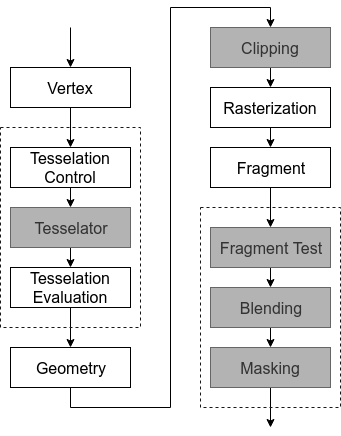
\includegraphics[width=0.3\textwidth]{opengl-pipeline.png}
  \end{center}
  \caption{The stages of the OpenGL rendering pipeline. White boxes represent stages that can be customised with shader code.}
  \label{fig:opengl-pipeline}
\end{figure}

For consistency, we refer to a step within the hardware rendering pipeline as a ``stage'', an invocation of the hardware pipeline as a ``pass'', and all invocations of the hardware pipeline to produce an image as a ``frame''. \\

Each of the customisable stages accepts only a single shader for each pass, making it difficult to separate, encapsulate, and ultimately combine behaviour. Furthermore, the steps required in order to change the shaders and shader inputs can be non-trivial and expensive to execute. \\

\begin{figure}[h]
  \begin{center}
    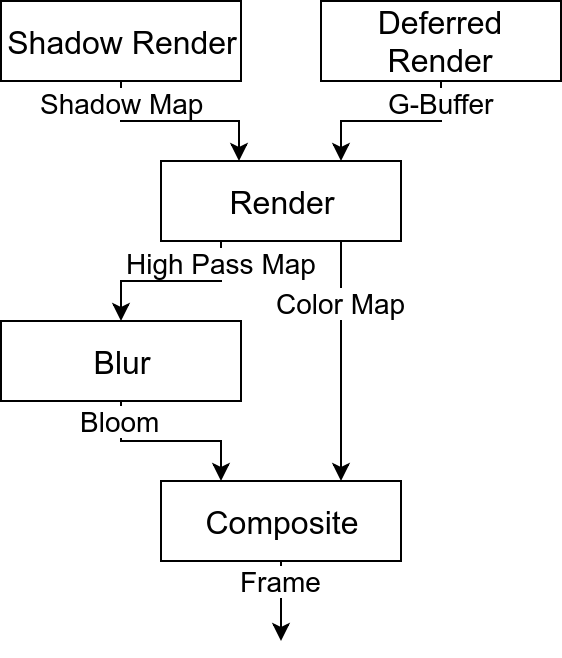
\includegraphics[width=0.3\textwidth]{render-pipeline.png}
  \end{center}
  \caption{A sample frame pipeline with shadow mapping, deferred rendering, and bloom. Each box represents a pass and each edge a texture buffer.}
  \label{fig:render-pipeline}
\end{figure}

Managing this graphics state and the order of rendering can be very complicated for modern requirements. Rendering a frame often requires a multitude of passes, each with their own parameters and shared data. The rendering of each object within a pass can also differ, leading to even more state that needs to be correctly managed. \\

This complexity results in a difficult challenge for modularity. We attempt to solve this challenge through several systems:

\begin{itemize}
\item A protocol for communicating information between a pass and the objects rendered within.
\item A protocol to connect the inputs, outputs, and parameters of different passes.
\item An algorithm to automatically allocate shared textures used as buffers between passes.
\end{itemize}

\section{Related Work}\label{relatedwork}
Courreges\cite{gtav} presents an in-depth analysis of the rendering procedure employed by the modern, high-production game GTA V. It illustrates the many passes to produce a final image, as well as their data dependencies. \\

Harada et al.'s work on Forward+\cite{forward+}\cite{forward+talk} also clearly illustrates the need for systems that support multi-pass rendering pipelines with complex data interaction schemes. \\

Gyrling\cite{fibers} presents an overview of the techniques used to perform parallel rendering in Naughty Dog's private game engine. Individual stages within a pass, render passes of a frame, and multiple frame renderings are divided up into many small jobs that can run in parallel and are synchronised using counters on a shared structure. How rendering logic requirements are communicated is however not explained. \\

The case study of the Unity game engine by Messaoudi et al\cite{unity} shows the availability of a set of fixed rendering pipelines that can be customised to a very limited extent with custom shaders. These shaders must fit into Unity's existing lighting and overall rendering model. While Unity does allow building a custom pipeline via their Scriptable Rendering Pipeline\cite{unitycustom}, they do not seem to offer any specific encapsulation or modularity features. \\

The work by He et al.\cite{components} introduces a framework for general encapsulation of shaders and their parameters into structures that minimise the overhead of changing GPU state while retaining the ability to dynamically compose shader parts. They do however not create a distinction between properties for rendering an object and for those for rendering an overall pass. \\

Foley et al.'s work on Spark\cite{spark} presents a high-level graph-based system for defining reusable and composable shader components. Their system shows a much more distanced view of the underlying graphics hardware than we attempt. Similar to He's work, they do not present a separation between object logic and pass logic. \\

In our previous work\cite{glsloop} we introduce a system to tie shader code to classes and to compose behaviour through inheritance. We make use of this system and extend it to allow further control over rendering behaviour in individual passes.

\section{Overview}\label{overview}
The system is composed of three distinct entities: shader objects, shader passes, and pipelines. Both shader objects and shader passes encapsulate rendering logic. The pipeline, on the other hand, represents the assembly of a complete frame, and only influences rendering in the sense that it tracks which passes to run in what order. \\

Due to the restrictions of the rendering pipeline of OpenGL, the combination of the render logic of objects and of passes is not trivial. We present a protocol to solve this difficulty in \hyperref[passes]{section 4}. \\

In \hyperref[pipelines]{section 5} we present a protocol for representing input and output information of a pass and for connecting these inputs and outputs between passes together. \\

Due to the complex interactions between passes in a pipeline, allocation of intermediary buffer textures is error-prone and tedious. We present algorithms to automate this in \hyperref[allocation]{section 6}. \\

Finally, in \hyperref[concept]{section 7} we show the results of implementing a medium-sized pipeline using these techniques.

\section{Passes}\label{passes}
A shader pass should encapsulate the logic for drawing objects in a certain way. In order to accomplish its task, the pass needs to be able to partially or fully control the shaders of objects. For instance, an object should still be able to have control over how its vertices are constructed and what materials and textures are applied to it. The shader pass should be able to make use of this information if it needs to, or discard it completely if unneeded. \\

In order to permit this amount of control, we make use of the shader composition capabilities that we presented in our previous work\cite{glsloop}. This technique allows us to combine pieces of OpenGL Shader Language (GLSL) code. On top of this shader combination sits a new protocol to control the interaction between shader passes and objects. \\

\begin{listing}[h]
\begin{minted}[fontsize=\small]{common-lisp}
(defclass shader-pass ()
  ()
  (:metaclass shader-pass-class))

(defgeneric register-object-for-pass (shader-pass object))
(defgeneric shader-program-for-pass (shader-pass object))
(defgeneric make-pass-shader-program (shader-pass object))
(defgeneric coerce-pass-shader (shader-pass object stage))
(defgeneric render-with (shader-pass object))
(defgeneric render (object target))
\end{minted}
\caption{The protocol for shader passes.}
\label{lst:pass}
\end{listing}

For any object that should be rendered using a given pass, first \code{register-object-for-pass} must be called. This call allows the pass to prepare the shader program that will be used during rendering for this object. A shader program is an OpenGL resource that compiles the shaders for the stages of a pass together. Using \\ \code{shader-program-for-pass} this program can then later be retrieved. The shader program is important for objects to access, as it allows them to set values for ``uniform'' variables that are used in the shader code. \\

\code{register-object-for-pass} calls \code{make-pass-shader-program} to compute this program, and registers it internally in the shader pass so that it can be retrieved later. If the shader pass would like to retain complete control over how each object is drawn, it would forego this call and instead generate its own shader program. Doing so is especially useful for post-processing effects that don't render any objects at all, and instead simply operate on textures that are output by previous passes. \\

\code{make-pass-shader-program} gathers all the shader sources for a program using \code{coerce-pass-shader} and then generates a representation for an OpenGL shader program. This representation also includes additional information such as the data buffers used. \\

\code{coerce-pass-shader} computes the effective shader source for a particular shader stage or type. Typically this computation simply involves the combination of the shader sources of both the shader pass and of the object, for the given shader type. We perform this combination using the same parsing and code walking strategy as we described in our previous work.\cite{glsloop} \\

Objects are typically rendered using the \code{render} function. Users are encouraged to add methods that specialise the behaviour and perform necessary setup, as well as to perform the final draw call for their custom object classes. For instance, a very primitive class could look as shown in \autoref{lst:simple-object}. \\

\begin{listing}[h]
\begin{minted}[fontsize=\small]{common-lisp}
(defclass simple-object ()
  ((vertex-array :accessor vertex-array)
  (:metaclass shader-class))

(defmethod render ((oject simple-object) target)
  (let ((vao (vertex-array object)))
    (gl:bind-vertex-array (gl-name vao))
    (%gl:draw-elements :triangles (size vao) :unsigned-int 0)))

(defmethod render :before ((object simple-object)
                           (pass shader-pass))
  (let ((program (shader-program-for-pass pass object)))
    (setf (uniform program "projection_matrix")
          (projection-matrix))))
\end{minted}
\caption{A simple object class and its render methods. The first method tells OpenGL to render a list of vertices. The second method sends the projection matrix to the GPU via a uniform variable.}
\label{lst:simple-object}
\end{listing}

This function is fine for allowing the object control over the behaviour. However, the pass cannot exert the same amount of control, due to the generic function's argument precedence. For example, if an \code{:around} method specialised on the object exists, a pass would not have any way of preventing it from firing, as its own \code{:around} method would be executed afterwards. We thus introduce another function with inverted argument order that is called first. \\

\code{render-with} thus exists mostly as an entry point to allow shader passes greater control over the rendering. Typically it will simply defer to \code{render}. This inversion is very important for shader passes that take all control away from the objects. \\

This protocol thus allows a great amount of control both over the effective shader code used to render an object, as well as the behaviour leading up towards the actual draw call for an object. \\

The overall protocol thus only invokes overhead for the dispatch of the \code{render-with}, \code{render}, and \code{shader-program-for-pass} generic functions for each rendered object per frame. All other functions are only invoked during loading, or in exceptional situations. In our use of the system so far we have not found this to impact performance significantly.

\section{Pipelines}\label{pipelines}
Shader passes not only retain information about how objects are drawn, but also about the input and output textures that a pass interacts with. For this reason, each shader pass is also a node in a graph, with distinct input and output ports.

\begin{listing}[h]
\begin{minted}[fontsize=\small]{common-lisp}
(defclass deferred-render (shader-pass)
  ((position-map :port-type input)
   (normal-map :port-type input)
   (albedo-map :port-type input)
   (color :port-type output))
  (:metaclass shader-pass-class)
\end{minted}
\caption{An outline of a deferred rendering pass, taking position-, normal-, and albedo-map textures as input, producing a single color texture as output.}
\label{lst:deferred-render}
\end{listing}

An example of such a pass is illustrated in \autoref{lst:deferred-render}. The ports are modelled as slots of the class that carry additional metadata, requiring a new metaclass. A slot with a port-type will not only hold a texture for its value, but also retain information about how it is connected to other passes. Using slots in this manner also allows us to inherit ports from other classes, and thus combine behaviour alongside the shader source code. \\

For the sake of brevity and ease of explanation, we have left out the details of texture constraints in these code samples. Nevertheless, constraining the features of textures tied to the ports is important, and we discuss the technique for dealing with that in \hyperref[allocation]{section 6}. \\

\begin{listing}[h]
\begin{minted}[fontsize=\small]{common-lisp}
(defclass shadow-render (shader-pass)
  ((shadow-map :port-type input)
   (color :port-type output))
  (:metaclass shader-pass-class))
\end{minted}
\caption{An outline of a shadow rendering pass, taking into account the information from a shadow-map to render shadows onto the output color texture.}
\label{lst:shadow-render}
\end{listing}

\begin{listing}[h]
\begin{minted}[fontsize=\small]{common-lisp}
(defclass high-pass-render (shader-pass)
  ((high-pass :port-type output))
  (:metaclass shader-pass-class))
\end{minted}
\caption{An outline of a high-pass renderer, which splices off colours of a high intensity into a high-pass output texture.}
\label{lst:high-pass}
\end{listing}

For instance, the ``Deferred Render'' pass shown in \autoref{fig:render-pipeline} is created by combining the passes illustrated in \autoref{lst:deferred-render}, \autoref{lst:shadow-render}, and \autoref{lst:high-pass} through inheritance. \\

When assembling a pipeline, we can then connect these ports together, in order to dictate how the various output textures generated by a pass are used as inputs for other passes. As an example, the pipeline from \autoref{fig:render-pipeline} is created in \autoref{lst:pipeline}. \\

\begin{listing}[h]
\begin{minted}[fontsize=\small]{common-lisp}
(let ((pipeline (make-pipeline))
      (shadow (make-instance 'shadow-map-pass))
      (geometry (make-instance 'geometry-pass))
      (deferred (make-instance 'deferred+shadow-pass))
      (blur (make-instance 'gaussian-blur-pass))
      (composite (make-instance 'composite-pass)))
  (connect (port shadow 'shadow-map) 
           (port deferred 'shadow-map) pipeline)
  (connect (port geometry 'position-map)
           (port deferred 'position-map) pipeline)
  (connect (port geometry 'normal-map)
           (port deferred 'normal-map) pipeline)
  (connect (port geometry 'albedo-map)
           (port deferred 'albedo-map) pipeline)
  (connect (port deferred 'high-pass)
           (port blur 'previous-pass) pipeline)
  (connect (port deferred 'color)
           (port composite 'color) pipeline)
  (connect (port blur 'color)
           (port composite 'bloom) pipeline)
  (prepare pipeline))
\end{minted}
\caption{An assembly of the pipeline shown in \autoref{fig:render-pipeline}.}
\label{lst:pipeline}
\end{listing}

The pipeline object itself retains information on the order in which the passes should be executed, and keeps track of the textures that are allocated in order to run the passes. How this information is computed is described in \hyperref[allocation]{section 6}. \\

The procedure to actually render objects with this pipeline technique is then as follows:

\begin{step}
\item Create a pipeline object and instances of the desired shader passes.
\item Connect the ports of the shader passes.
\item Prepare the pipeline to allocate the needed resources.
\item Create instances of the desired objects.
\item Register each object with each pass.
\item Call \code{render} on the pipeline with a collection of all objects to draw.
\item The output texture of the output port of the last shader pass in the pipeline will contain the finished frame.
\end{step}

The completed frame can then be blitted onto the screen, or be used as the input for another computation.

\section{Allocation}\label{allocation}
In order to prepare the shader pipeline, several resources need to be allocated. Each shader stage needs a ``framebuffer,'' an OpenGL resource that allows one to render to off-screen textures. These framebuffers then need to have the required textures to render allocated as well. As each input and output from a pass can specify constraints on the features of the texture, these constraints must be matched up for any connecting edges as well. Finally, in order to minimise memory usage, we would like to re-use textures where possible. \\

Thus, the allocation proceeds in three phases: reconciling texture constraints on edges between passes, computing how textures are shared between passes, and finally constructing all the necessary resources with the previously gathered information.

\subsection{Constraint Merging}\label{texture-constraints}
OpenGL textures include a massive amount of information\cite{texparameter}\cite{teximage2d}. When two ports are connected that specify different constraints on the texture properties, a join must be performed. A wide range of the texture property values are fundamentally incompatible, meaning that a lot of the logic can simply error. However, other options require more complicated joining logic. For simplicity and brevity, we will focus on the join operator for a single texture property here: the internal format. The internal format is arguably the most important property. This property specifies how many colour channels the texture has, how many bits of precision each channel has, which format each channel has, as well as whether the texture is compressed or has sRGB gamma normalisation applied. \\

The list of specified texture formats is quite large\cite{texinternalformat}. Unfortunately OpenGL does not give us an interface to handle these formats in a way that lets us pick the individual features easily. Instead, each format is represented by a constant whose value has no relation to the features that format includes. This representation means that we first need to destructure each format name into a list of features: \\

\begin{itemize}
\item \code{R}, \code{G}, \code{B}, \code{A} How many bits to use for each channel, and the format of the channel (normalised, float, integer, unsigned integer).
\item \code{depth} How many bits to use for the depth channel.
\item \code{stencil} How many bits to use for the stencil channel.
\item \code{shared} Whether bits are shared across the channels, and if so how many.
\item \code{features} Whether the format has compression, sRGB, RGTC, BPTC, SNORM, or UNORM features.
\end{itemize}

Once the texture format specifications are destructured, we can perform a join as follows.

\begin{step}
\item If the \code{features} and sharing are not the same, a join is impossible.
\item The \code{features} list of the output spec is set to the same as either of the specs.
\item If both include a \code{depth} component:
  \begin{step}
  \item The \code{depth} feature is set to the join of both.
  \item If either include a \code{stencil} feature, the \code{stencil} feature is set to the join of both.
  \end{step}
\item If both include a \code{stencil} component:
  \begin{step}
  \item The \code{stencil} feature is set to the join of both.
  \end{step}
\item If neither include a \code{depth} component:
  \begin{step}
  \item The \code{R} feature is set to the join of both.
  \item The \code{G} feature is set to the join of both.
  \item The \code{B} feature is set to the join of both.
  \item The \code{A} feature is set to the join of both.
  \end{step}
\item Otherwise a join is impossible.
\end{step}

Wherein the ``join of both'' is computed as the join of two channel formats as follows.

\begin{step}
\item If both include the format:
  \begin{step}
  \item If the channel format is not the same, a join is impossible.
  \item The channel bit depth is set to the maximum of both.
  \end{step}
\item If one includes the format, that format is returned.
\item Otherwise, the absence of the channel is indicated.
\end{step}

If the join is successful, we then re-encode the texture format specification into OpenGL's constant and use this constant in the real texture specification. Note that this join could produce texture format specifications that are not legal according to the OpenGL specification. However, this can only occur if one of the specifications to join is already illegal. We thus deem it unnecessary to handle such cases.

\subsection{Port Allocation}\label{port-allocation}
In compilers, allocation of a graph of variables with use-relations is typically handled with a graph colouring algorithm. However, since we represent our graph in a different fashion than usual, with nodes having multiple distinct ports on which edges are connected, we devised a different kind of colouring algorithm to maximise texture sharing. \\

Given a set of nodes the allocation algorithm proceeds as follows.

\begin{step}
\item The set of unique texture specifications is computed by joining each port's texture specification with every other and comparing for equality.
\item For each unique texture specification T:
  \begin{step}
  \item The nodes are sorted topologically.
  \item The number of colours is set to 0.
  \item For each node N:
    \begin{step}
    \item For each output port P of N:
      \begin{step}
      \item If P's texture specification is joinable with T...
      \item The number of colours is increased
      \end{step}
    \end{step}
  \item An array is allocated to fit the number of colours. Each index of the array represents a colour and each value at the index whether the colour is currently available or unavailable.
  \item For each node N in \emph{reverse order}:
    \begin{step}
    \item For each input port P of N:
      \begin{step}
      \item For each neighbour port O of P:
        \begin{step}
        \item If O's texture specification is joinable with T...
        \item and O does not yet have a colour...
        \item The first available colour is assigned to O.
        \item This colour is marked as unavailable.
        \end{step}
      \end{step}
    \item For each non-input port P of N:
      \begin{step}
      \item If P's texture specification is joinable with T...
      \item and P does not yet have a colour...
      \item The first available colour is assigned to P.
      \item This colour is marked as unavailable.
      \end{step}
    \item For each port P of N:
      \begin{step}
      \item If P's texture specification is joinable with T...
      \item and P has a colour...
      \item P's colour is marked as available.
      \end{step}
    \end{step}
  \end{step}
\end{step}

In other words, the algorithm proceeds backwards from the last node in the graph, marking output ports of predecessors with unique colours, then marking unconnected ports with unique colours, and finally marking all colours at the node's own output ports as available again. We repeat this process for each unique texture specification, each time ensuring we only consider ports that share that texture specification. \\

This algorithm is by no means efficient, but since pipeline allocation only has to happen during loading phases, we currently do not consider this to be a big problem. We also have not performed any analysis as to whether the algorithm produces optimal allocation results in every case.\\

Unfortunately printed documents cannot yet display animations, so illustrating the algorithm in motion is not possible directly in the document. However, a brief animation of the pipeline illustrated in \autoref{fig:render-pipeline} is available online: \\

\href{https://raw.githubusercontent.com/Shinmera/talks/master/els2019-shader-pipeline/pipeline-allocation.gif}{https://raw.githubusercontent.com/Shinmera/talks/master/\\els2019-shader-pipeline/pipeline-allocation.gif} \\

With this algorithm we reduce the number of necessary textures to allocate down to five. With a primitive allocation of one texture per output, we would instead end up with seven textures. Note that the shadow map output is not assigned, as it requires a different type of texture from the rest -- a depth texture. This texture would be allocated in a second pass.

\section{Proof of Concept}\label{concept}
As a proof of concept we have implemented these protocols and mechanisms, as well as the passes shown in \autoref{fig:render-pipeline}. As the code required to do so is quite lengthy and involved, and the graphics techniques used are beyond the scope of this paper, we will omit the code. The relevant outline of the passes and the pipeline involved has already been shown in \hyperref[pipelines]{section 5}. \\

Nevertheless, you can find the complete code online at the following pages: \\
\url{https://github.com/Shirakumo/trial/blob/b889d50/deferred.lisp} \\
\url{https://github.com/Shirakumo/trial/blob/b889d50/hdr.lisp} \\
\url{https://github.com/Shirakumo/trial/blob/b889d50/shadow-map.lisp} \\
\url{https://github.com/Shirakumo/trial/blob/b889d50/workbench.lisp} \\

\autoref{fig:pipeline-gbuffer}, \autoref{fig:pipeline-shadow}, \autoref{fig:pipeline-lighting}, \autoref{fig:pipeline-blur}, and \autoref{fig:pipeline-frame} show the output textures produced by the various stages for a simple scene.

\begin{figure}[h]
  \begin{center}
    \begin{minipage}{.2\textwidth}
      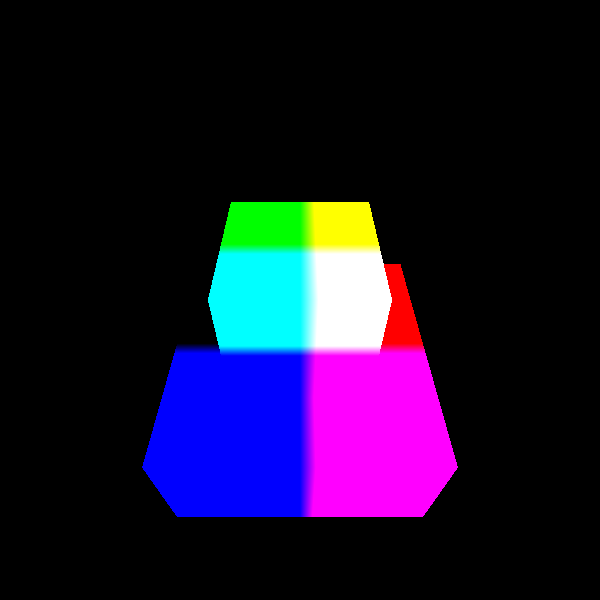
\includegraphics[width=1.0\textwidth]{pipeline-position.png}
    \end{minipage}
    \begin{minipage}{.2\textwidth}
      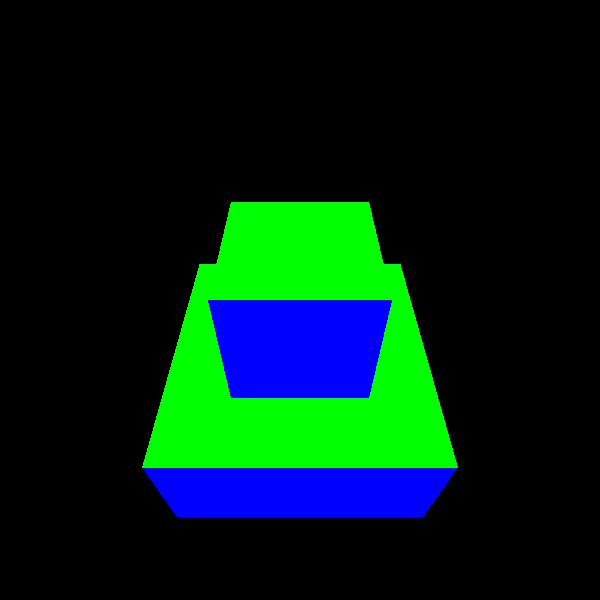
\includegraphics[width=1.0\textwidth]{pipeline-normal.png}
    \end{minipage}
    \vskip0.04cm
    \begin{minipage}{.2\textwidth}
      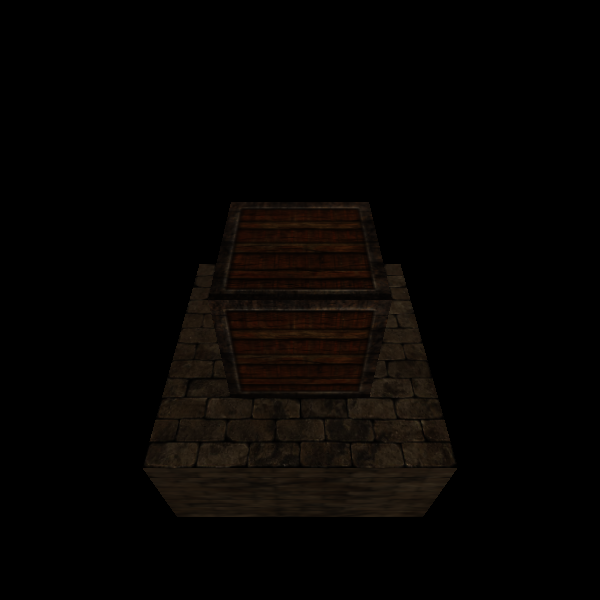
\includegraphics[width=1.0\textwidth]{pipeline-albedo.png}
    \end{minipage}
    \begin{minipage}{.2\textwidth}
      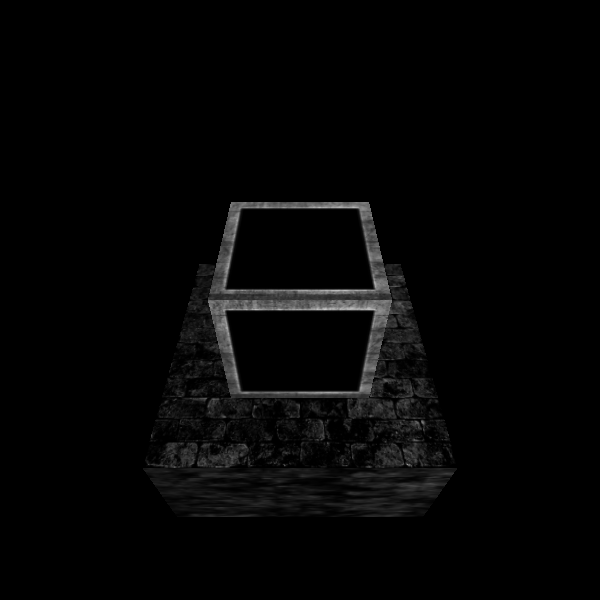
\includegraphics[width=1.0\textwidth]{pipeline-specular.png}
    \end{minipage}
  \end{center}
  \caption{The output of the geometry pass, producing a ``G-buffer'' composed out of a position- (top left), normal- (top right), albedo- (bottom left), and specular-map (bottom right).}
  \label{fig:pipeline-gbuffer}
\end{figure}

\begin{figure}[h]
  \begin{center}
    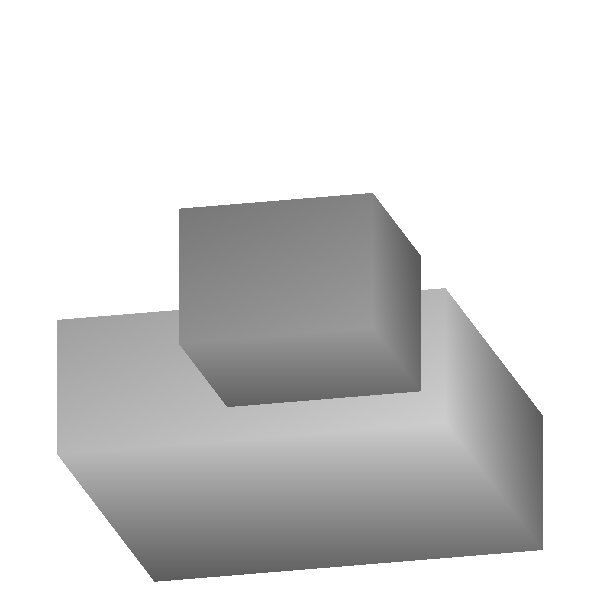
\includegraphics[width=0.2\textwidth]{pipeline-shadow.png}
  \end{center}
  \caption{The depth map produced by the shadow map pass. It shows the distance of surfaces from the point of view of the primary light source.}
  \label{fig:pipeline-shadow}
\end{figure}

\begin{figure}[h]
  \begin{center}
    \begin{minipage}{.2\textwidth}
      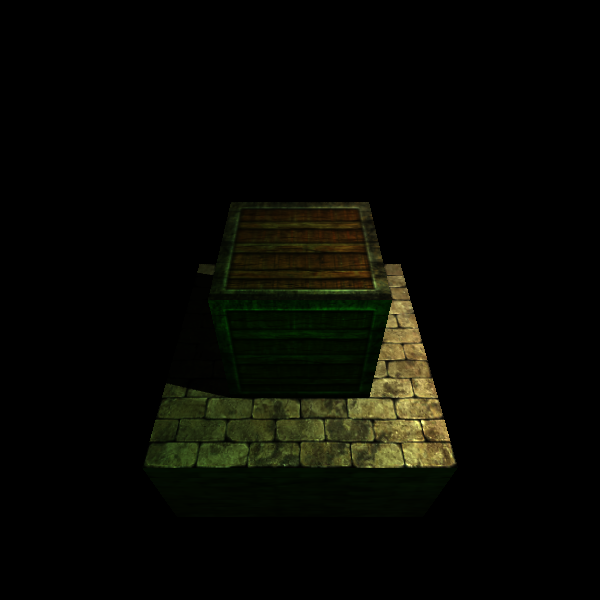
\includegraphics[width=1.0\textwidth]{pipeline-lighting.png}
    \end{minipage}
    \begin{minipage}{.2\textwidth}
      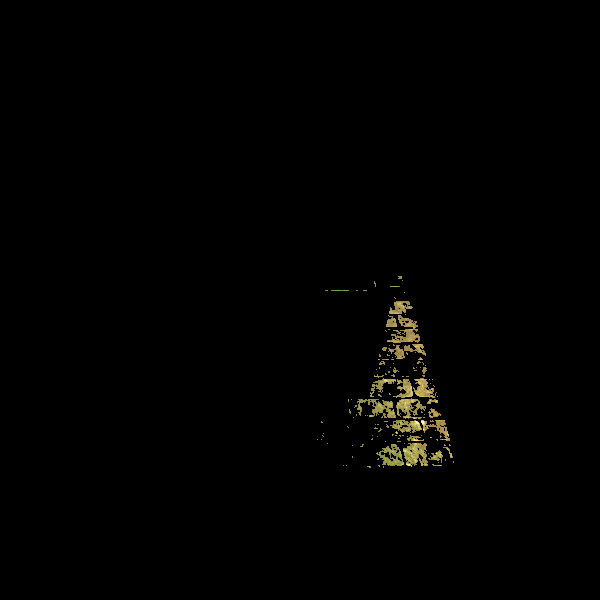
\includegraphics[width=1.0\textwidth]{pipeline-highpass.png}
    \end{minipage}
  \end{center}
  \caption{The color map (left) and the high-pass map (right) that is output by the deferred render pass. It combines the information from the G-buffer from \autoref{fig:pipeline-gbuffer}, the shadow-map from \autoref{fig:pipeline-shadow}, and information for lights to render an image. Note that due to gamma adjustments the image appears quite dark.}
  \label{fig:pipeline-lighting}
\end{figure}

\begin{figure}[h]
  \begin{center}
    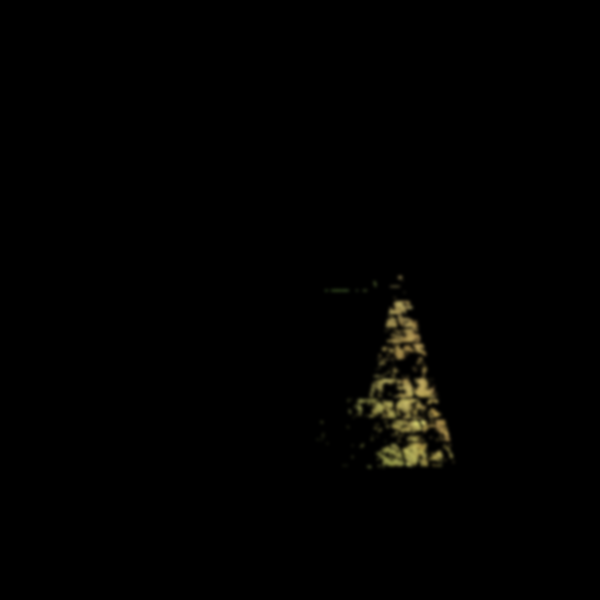
\includegraphics[width=0.2\textwidth]{pipeline-blur.png}
  \end{center}
  \caption{The blurred high-pass from \autoref{fig:pipeline-lighting} produced by the gaussian blur pass. This is used to produce an effect called bloom in the final composite pass.}
  \label{fig:pipeline-blur}
\end{figure}

\begin{figure}[h]
  \begin{center}
    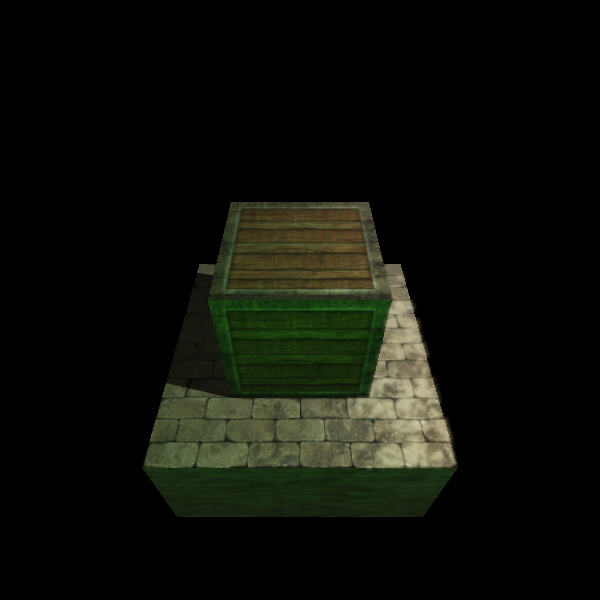
\includegraphics[width=0.4\textwidth]{pipeline-frame.png}
  \end{center}
  \caption{The final output frame that is produced by adding together the bloom texture from \autoref{fig:pipeline-blur} and the standard colour texture from \autoref{fig:pipeline-lighting}. Gamma adjustment and High Dynamic Range reduction are used for colour normalisation.}
  \label{fig:pipeline-frame}
\end{figure}

\newpage ~ % Fucking latex, give me a new page.

\section{Conclusion}\label{conclusion}
We have presented a system to handle the separation between objects that should be rendered, and the way in which they should be rendered. By using a protocol for the interaction between such objects and passes, we are capable of controlling and combining a variety of rendering behaviours. With an additional protocol and set of algorithms we also present a high-level view of rendering pipelines, allowing users to conveniently compose effects to produce complicated scenes. \\

These protocols and algorithms are largely generic enough that they could also be adapted for use in other languages and systems. However, we believe that the Common Lisp Object System gives us a set of very convenient tools to make everything feel more natural and more integrated with the rest of the system than other environments would allow us to do. \\

Finally, we have demonstrated the capability of this system by constructing a real-time rendering system out of individual, modular pieces of code.

\section{Further Work}\label{further-work}
Currently there exist several restrictions in our framework. \\

Most severe is that there is no standardised protocol to communicate capabilities and data between objects and passes. This restriction means that, for instance, an object that does not possess texturing has no way of communicating this to a shader pass that might need to render it. Currently this problem is partially solved by introducing a mandatory superclass that objects need to be a subtype of, if they want to be renderable under a given pass. This superclass then loosely defines the interaction. However, this additional class does not solve issues of compatibility of shader code used by the object and by the shader pass. In order to properly resolve this restriction, we currently see two required features: \\

Shader source merging must be aware of uses-relations, meaning that the code walker must track where variables, functions, and types are used and reorder the definitions and declarations in such a way that the dependencies are fulfilled. In GLSL, variables, functions, and types cannot be referenced before they are declared, requiring this reordering step. With this problem solved, shader code could be written in such a way to be more amiable towards combination and manipulation by external code. \\

GLSL's limited expressiveness makes it very difficult to figure out relations between code and how to properly combine pieces. A more high-level language, as is used in other frameworks like Spark\cite{spark} or Shader Components\cite{components}, should be introduced to allow a more convenient way to declare and write shaders, objects, and passes. With a higher-level language, a compiler could more easily figure out how to combine features and reconcile differences between pieces of code. \\

Another restriction is that there is currently no way to encapsulate GLSL code other than associating it with a class, which is a rather heavy-weight operation. It would be far more useful to introduce a library mechanism that allows the definition of standalone shader functions, which can then be required by shader classes.

\section{Acknowledgements}\label{acknowledgements}
I would like to thank Michal ``phoe'' Herda, Robert Strandh, Michael Reis, and all the people that will review this paper. Your name could be here!

\section{Implementation}\label{implementation}
An implementation of the proposed system can be found at \\
\url{https://github.com/Shirakumo/trial/blob/b889d50/shader-pass.lisp} \\
\url{https://github.com/Shirakumo/trial/blob/b889d50/pipeline.lisp} \\
\url{https://github.com/Shinmera/flow} \\

\bibliography{paper}
\end{document}

%%% Local Variables:
%%% mode: latex
%%% TeX-command-extra-options: "-shell-escape"
%%% TeX-master: t
%%% TeX-engine: luatex
%%% End:
